\chapter{总结与展望}

% 官方要求：对机器人各项功能点进行测试验收，记录测试环境、测试设备等信息，并总结研发过程中的经验与教训。

\section{测试记录}

在本赛季的研发过程中，我们对空中机器人的各项功能点进行了多轮测试与验收，主要测试记录如\tabref{tab:整机测试记录}所示。

\begin{longtable}[htbp!]{ m{1cm}<{\centering}  m{1.6cm}<{\centering}  m{2.3cm}<{\centering}  m{4.9cm}<{\centering}  m{5.6cm}<{\centering} }
\hline
序号 & 测试阶段 & 测试内容 & 测试结果（量化） \\
\hline
\endfirsthead
\hline
序号 & 测试阶段 & 测试内容 & 测试结果（量化） \\
\hline
\endhead
\hline
\multicolumn{5}{r}{接下页}
\endfoot
\caption{空中机器人整机测试记录}
\label{tab:整机测试记录}
\endlastfoot
 \hline
 1 & 机臂折叠 & 初版折叠件拆装与强度 & 折叠时间单人 5 分钟；运输中易断裂，需优化 \\
 \hline
 2 & 机臂折叠 & 终版折叠件拆装与强度 & 折叠时间单人 1 分 30 秒，单件仅 50g，国赛期间无损坏 \\
 \hline
 3 & 桨保 & 一体式桨保维护性 & 检修内部需整体拆卸，维护不便，改为分体式 \\
 \hline
 4 & 桨保 & 分体式桨保强度与减重 & 四件合计约 1.6kg，维护时仅需拆卸对应侧，强度满足要求 \\
 \hline
 5 & 发射机构 & 单发限位与定心效果 & 轴承式单发限位较拉簧弹速更稳定，定心效果更佳 \\
 \hline
 6 & 发射机构 & 曲面摩擦轮散布测试 & 更换 M2006 曲面摩擦轮后散布显著改善 \\
 \hline
 7 & 供弹 & 弹链与拨盘卡弹率 & 干性润滑油与挡边研磨后，1000 发卡弹次数小于等于 1 \\
 \hline
 8 & 云台 & 元件布局迭代 & 横向双相机布局降低 Pitch 转动惯量，响应速度大幅改善 \\
 \hline
 9 & 动力系统 & 满载悬停与续航 & 好盈 8100UL + 3098 桨叶，满载约 18kg 稳定悬停，温度正常 \\
 \hline
 10 & 定位 & FAST-LIO 悬停精度 & 全场连续定位，高频位姿插值至 100Hz，悬停精度满足要求 \\
 \hline
\end{longtable}

\subsection{测试环境与设备}
\begin{itemize}
    \item 飞行测试在室内空旷场地进行，避免室外气流与光照对测试的干扰；
    \item 散布测试在固定发射测试架上进行，以机械固定方式稳定云台 Pitch/Yaw 轴，完全排除控制因素对机械精度的干扰；
    \item 定位与悬停测试在标准赛场空域模拟环境下进行，配合激光雷达、飞控日志与上位机调试器记录数据。
\end{itemize}

\section{研发迭代过程}

本赛季空中机器人经历了多轮设计迭代，主要版本演进如\tabref{tab:研发迭代过程}所示。

\begin{longtable}[htbp!]{ m{2.4cm}<{\centering}  m{9.4cm}<{\centering}  m{2.6cm}<{\centering} }
\hline
版本阶段 & 功能或性能说明 & 完成时间 \\
\hline
\endfirsthead
\hline
版本阶段 & 功能或性能说明 & 完成时间 \\
\hline
\endhead
\hline
\multicolumn{3}{r}{接下页}
\endfoot
\caption{空中机器人研发迭代过程}
\label{tab:研发迭代过程}
\endlastfoot
 \hline
 V1 & 完成初版折叠件与一体式桨保设计，完成机身中心板、机臂与弹仓结构设计 & 赛季前期 \\
 \hline
 V2 & 折叠件改用塞打转轴与手拧螺丝方案并加钢片补强；桨保改为分体式设计 & 中期 \\
 \hline
 V3 & 云台元件布局重构：横向双相机并架高，图传下移，小电脑后置，降低转动惯量 & 中期 \\
 \hline
 V4 & 发射机构迭代：摩擦轮电机由 M3508 更换为 M2006，摩擦轮改为曲面结构 & 中后期 \\
 \hline
 V5 & 单发限位由拉簧式改为轴承式，完成云台、发射、定位与软件联调 & 后期 \\
 \hline
\end{longtable}

\section{重点问题解决记录}

研发过程中遇到的问题及解决方案总结如\tabref{tab:重点问题解决}所示。

\begin{longtable}[htbp!]{ m{3.2cm}<{\centering}  m{4.8cm}<{\centering}  m{6.4cm}<{\centering} }
\hline
问题描述 & 问题产生原因 & 解决方案与效果 \\
\hline
\endfirsthead
\hline
问题描述 & 问题产生原因 & 解决方案与效果 \\
\hline
\endhead
\hline
\multicolumn{3}{r}{接下页}
\endfoot
\caption{空中机器人重点问题解决记录}
\label{tab:重点问题解决}
\endlastfoot
 \hline
 初版折叠件运输中容易断裂 & 拆装复杂、结构强度不足 & 采用塞打做转轴、手拧螺丝实现折叠，外侧垫钢片降低对碳板压强；国赛期间无损坏 \\
 \hline
 弹链供弹卡顿 & 弹链阻力大、拨盘挡边与弹丸相切角不佳 & 涂抹干性润滑油，调整挡边长度并研磨相切角，1000 发卡弹次数小于等于 1 \\
 \hline
 一体式桨保检修困难 & 中心板与飞控被桨保覆盖 & 改为分体式桨保，独立安装，维护时仅拆卸对应侧，大幅提升维护效率 \\
 \hline
 雷达震动影响定位精度 & 雷达固定刚度不足 & 采用纳米胶与电工胶将雷达粘贴于海绵垫减震，效果最佳且无过大机械位移 \\
 \hline
 摩擦轮 M3508 体积重量大 & 旧方案针对地面发射机构选型 & 更换为 M2006 电机与曲面摩擦轮，减重并改善定心度，散布显著改善 \\
 \hline
\end{longtable}

\section{总结与展望}

本赛季我们围绕"安全飞行、永不坠机"的总体目标，完成了可折叠机臂与分体式桨保、大角度双轴云台、高精度发射系统、硬件电源树、嵌入式软件与视觉导航算法的设计与联调，基本实现了绪论中提出的分级设计目标。在研发过程中，"轻量化与结构强度"、"稳定悬停与精准打击"、"定位可靠性与飞行安全"始终是贯穿整机的三条主线，任何一环的缺失都会在赛场上被放大。

参考仲恺奇点、深技大悍匠等强队的开源报告\cite{zhongkai_qidian_drone_2026,sztu_hanjiang_drone_2026}，本赛季各队空中机器人的作战数据（\figref{fig:比赛数据}）表明，稳定可靠的空中机器人已成为赛场上不可忽视的核心战力；同时，2025 赛季各赛区空中机器人坠机率居高不下的统计也提醒我们，可靠性仍是空中机器人区别于地面兵种的最大挑战。

\begin{figure}[hbtp!]
    \centering
    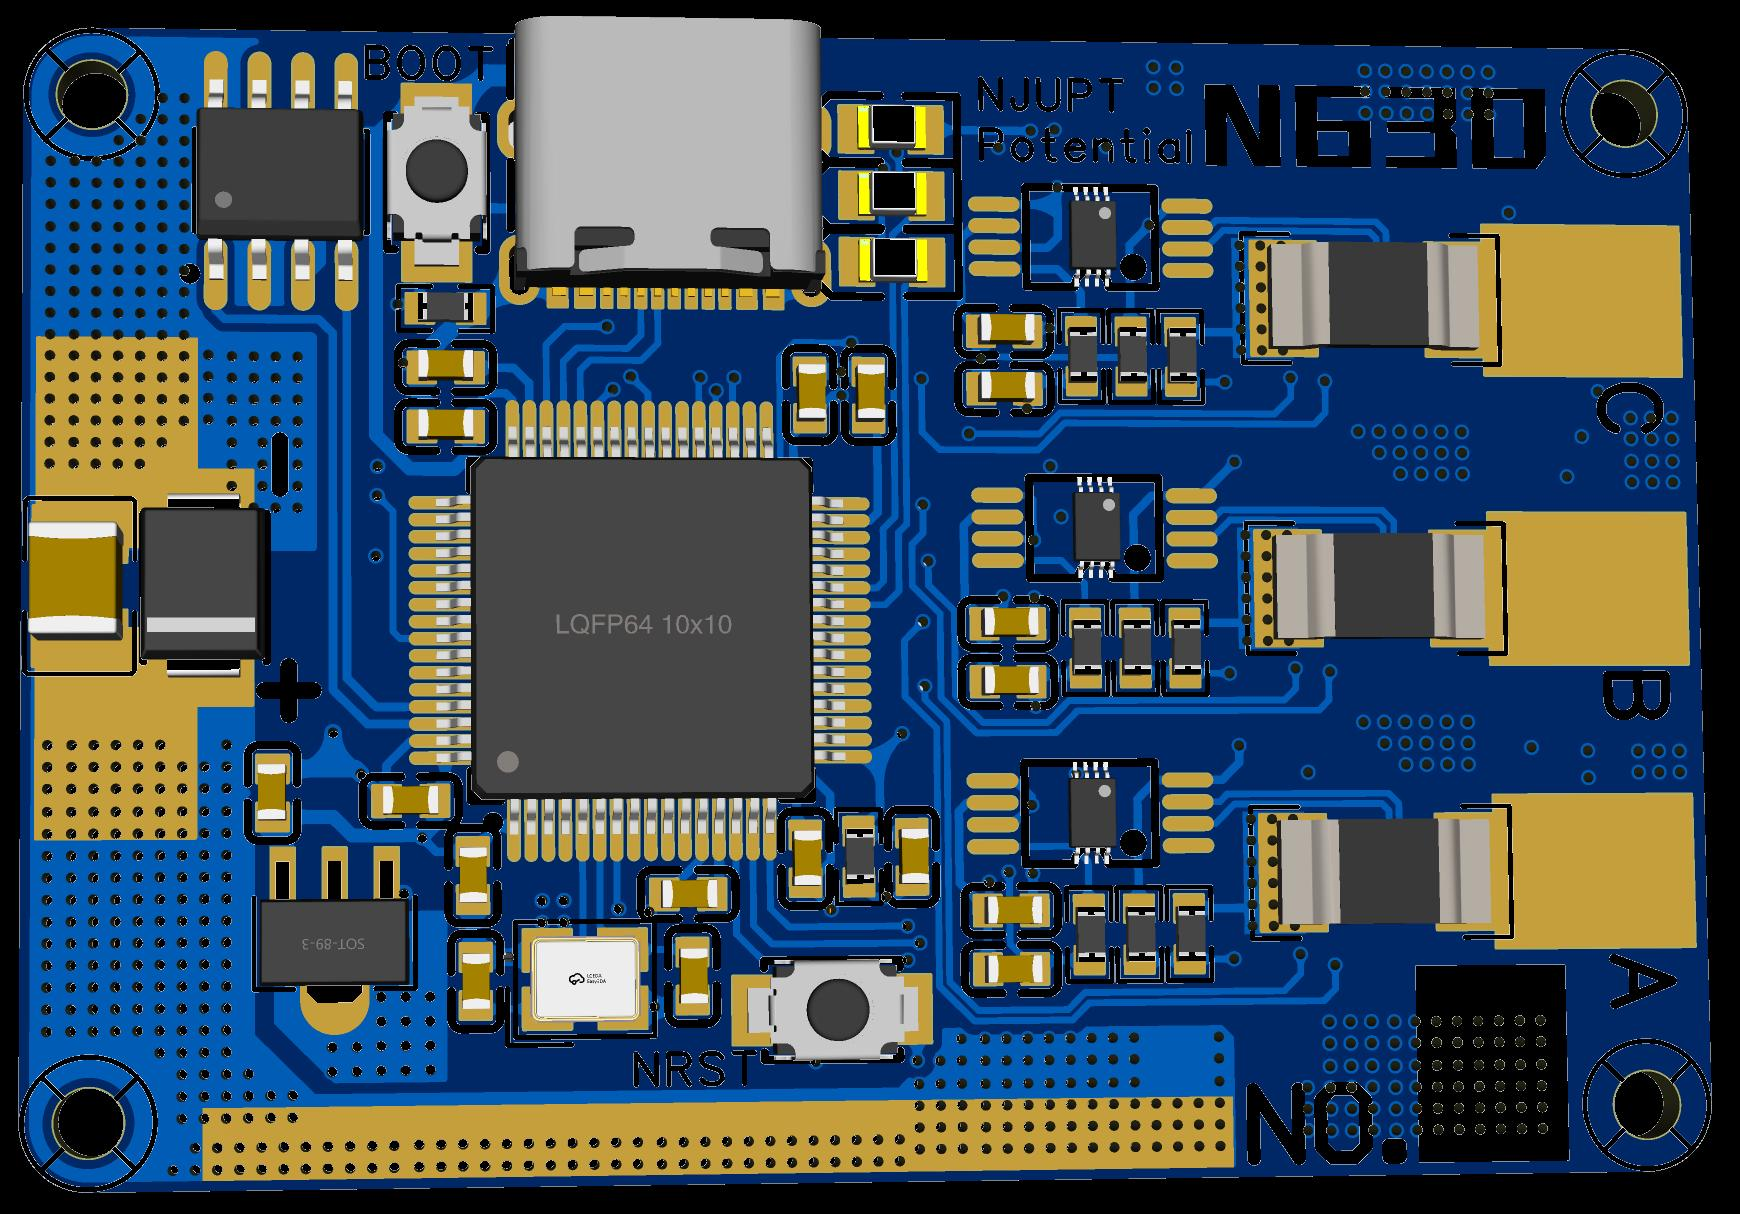
\includegraphics[width=0.7\linewidth]{figure/5_总结与展望/2026南部赛区比赛数据.png}
    \caption{2026 赛季南部赛区空中机器人比赛数据示例（图源：仲恺奇点战队开源报告\cite{zhongkai_qidian_drone_2026}）}
    \label{fig:比赛数据}
\end{figure}

下一赛季，我们计划在以下方向继续探索：
\begin{itemize}
    \item \textbf{进一步轻量化}：探索反桨方案与更轻的动力、供电系统，降低桨盘载荷，延长续航并提高机动性；
    \item \textbf{提高结构可靠性}：完善模块化快拆设计，缩短故障后的检修时间，降低坠机概率；
    \item \textbf{强化自瞄与飞行协同}：继续推进基于定位里程计的自运动补偿等实验链，提高高动态下的打击精度；
    \item \textbf{探索更多战术可能}：在满足规则的框架下，探索开能量机关、空地协同等更多空中机器人的战术价值。
\end{itemize}
